\section{Energy Resolution of the XENON100 Detector}
\label{secEnergyResolution}

\begin{figure}[!b]
\centering
\subfigure[]{
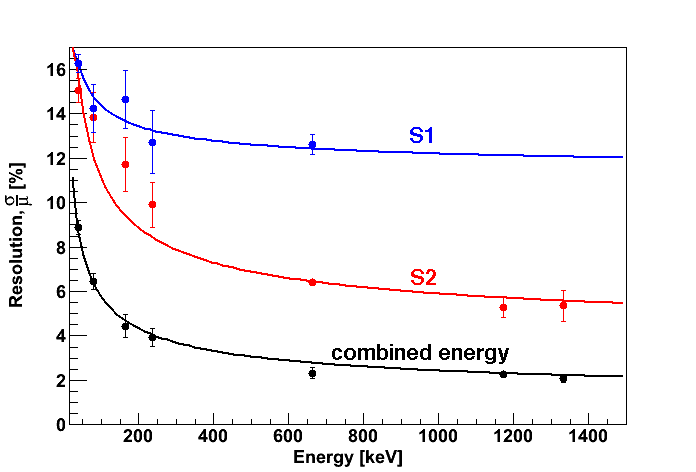
\includegraphics[width=0.475\linewidth]{plots/EnergyResolution/ResolutionFunctions_withEmpiricalCorrect_withLabels.png}
\label{figEnergyResolution_1}}
\subfigure[]{
%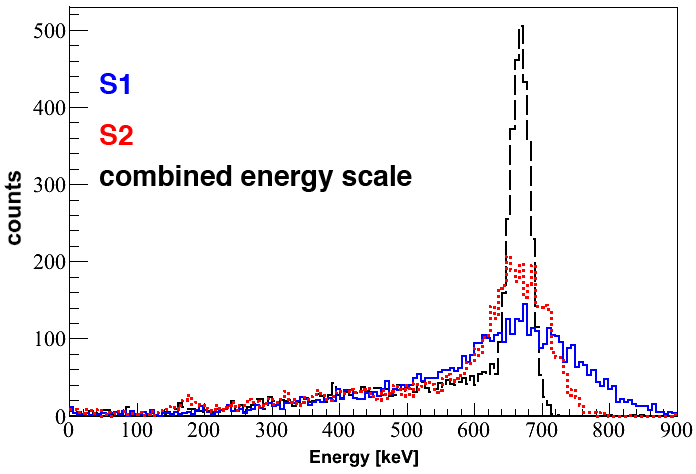
\includegraphics[width=0.45\linewidth]{plots/EnergyResolution/SpectrumDifferentScales_withLabels.png}
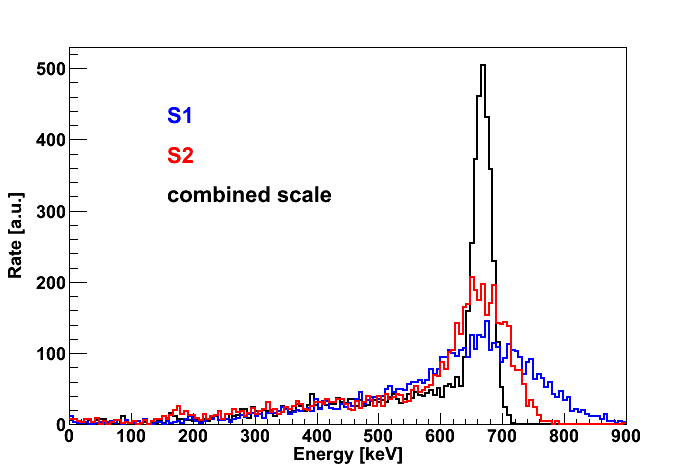
\includegraphics[width=0.475\linewidth]{plots/EnergyResolution/CsSpectrumDifferentScales.png}
\label{figEnergyResolution_2}}
\caption[XENON100 energy resolution as a function of energy, and $^{137}$Cs spectra in different energy scales]{XENON100 energy resolution as a function of energy (b), and $^{137}$Cs spectra in different energy scales (a). The $^{137}$Cs data point is slightly offset from the trend, which is probably an effect of the difference in the event spatial distribution and non-uniform response within the TPC.}
\label{figEnergyResolution}
\end{figure}

The energy resolution depends on the intrinsic resolutions of the scintillation and ionization processes in liquid xenon, geometrical fluctuation of light collection, and statistical fluctuations of the number of photoelectrons $N_{\mathrm{PE}}$ produced in the PMTs by incident photons. The latter dominates the resolution due to the lower number of quanta involved. In addition, the resolution $R$ includes the PMT gain variation (the average value measured on single PE spectrum is $\frac{\sigma_{\mathrm{gain}}}{\mathrm{gain}}$ = 52\%, see Section~\ref{secGainCalibration}) and is approximately equal to:
\begin{equation}
R = \sqrt{\frac{1+(\frac{\sigma_{\mathrm{gain}}}{\mathrm{gain}})^2}{N_{\mathrm{PE}}}}.
\end{equation}
Hence, the energy resolution improves with the number of measured photoelectrons (or incident energy), and is better when the proportional scintillation signal (S2) is considered, since it is two orders of magnitude larger than S1.

The energy resolution $R_{\mathrm{CES}}$ of the combined scale can be derived from equation (\ref{eqCES})~\cite{CES_Aprile}:
\begin{equation}
\label{eqCESresolution}
R_{\mathrm{CES}} = \sqrt{ \frac{\sin^2{\Theta} \cdot R_{\mathrm{S}_{1}}^2 + 2 \cdot \sin{\Theta} \cdot \cos{\Theta} \cdot R_{\mathrm{S}_{1}\mathrm{S}_{2}} + \cos^2{\Theta} \cdot R_{\mathrm{S}_2}^2 } { (\sin{\Theta} + \cos{\Theta})^{2} } },
\end{equation}
where $R_{\mathrm{S}_{1}}$ and $R_{\mathrm{S}_{2}}$ - energy resolutions from S1 and S2 spectra, respectively, and $R_{\mathrm{S}_{1}\mathrm{S}_{2}}$ - covariance between S1 and S2. The covariance $R_{\mathrm{S}_{1}\mathrm{S}_{2}}$ can be expressed in terms of a correlation coefficient $\rho_{\mathrm{S}_{1}\mathrm{S}_{2}}$, and its magnitude indicates the strength of anti-correlation between the two signals:
\begin{equation}
%\nonumber
\rho_{\mathrm{S}_{1}\mathrm{S}_{2}} = \frac{R_{\mathrm{S}_{1}\mathrm{S}_{2}}}{R_{\mathrm{S}_{1}} \cdot R_{\mathrm{S}_{2}}}.
\end{equation}
The value of the correlation coefficient $\rho_{\mathrm{S}_{1}\mathrm{S}_{2}}$ is between -0.7 to -0.9, indicating a very strong anti-correlation between S1 and S2.

The energy resolution has been measured at 40~keV, 80~keV, 164~keV, 236~keV, 662~keV, 1173~keV and 1332~keV, by a Gaussian fit to the peaks and calculation of the $\sigma$ of the distribution over its mean. The obtained data points have been fitted with a function of the form:
\begin{equation}
\label{eqFitResolution}
%\nonumber
f(E) = a + \frac{b}{\sqrt{E}},
\end{equation}
where $E$ - energy in [keV], $a$ and $b$ - constant factors. The results are shown in Fig.~\ref{figEnergyResolution_1}, with the functional forms:
\begin{equation}
%\nonumber
\frac{\sigma(E)}{E} \text{[\%]} = 11.2 + \frac{31.6}{\sqrt{E\ \text{[keV]}}} - \text{ for the energy scale based on S1},
\end{equation}
\begin{equation}
%\nonumber
\frac{\sigma(E)}{E} \text{[\%]} = 3.5 + \frac{75.9}{\sqrt{E\ \text{[keV]}}} - \text{ for the energy scale based on S2}, \
\end{equation}
%\begin{equation}
%\nonumber
%\frac{\sigma(E)}{E} \text{\%} = \frac{1.9}{\sqrt{E/MeV}} -\text{ for the combined energy scale}.
%\end{equation}
\begin{equation}
\label{eqResCES}
%\nonumber
\frac{\sigma(E)}{E} \text{[\%]} = 0.9 + \frac{48.5}{\sqrt{E\ \text{[keV]}}}  -\text{ for the combined energy scale}. \ \ \ \
\end{equation}

The results are shown in Fig.~\ref{figEnergyResolution_1}. The $^{137}$Cs data point is slightly offset from the trend. This is suspected to be due to the difference in the spatial distribution of the events and non-uniform response within the TPC. The $^{137}$Cs source has been always placed in one position, close to $Y$ = 0 on the right side, whereas $^{60}$Co has been placed in several positions around the detector, and the $^{241}$Am-Be calibration provides more a more uniform event distribution. The distribution of the energy resolution using only S2 signal is not described well with the function (\ref{eqFitResolution}), which might be an effect of the contribution of nuclear recoils in 40~keV and 80~keV lines described in Section~\ref{secCES}. 

The $^{137}$Cs energy spectra reconstructed using different scales are shown in Fig.~\ref{figEnergyResolution_2}, indicating the remarkable improvement of the detector resolution when using the combined scale. At 1~MeV, the resolution is 12.2\% using S1 signal, 5.9\% considering only S2 signal, and 1.9\% when the combined energy scale is used.



